\documentclass{article}
\usepackage{graphicx} % Required for inserting images
\usepackage[english, russian]{babel}
\usepackage{hyperref}
\usepackage[a4paper, margin=1in]{geometry} % Добавьте этот пакет для настройки полей

\title{Инструкция к программе имитации спасательных операций}
\author{Михаил Преображенский}
\date{September 2024}

\begin{document}

\maketitle
\tableofcontents

\newpage

\section{Установка программы}
Данная программа представляет из себя архив, состоящий из нескольких файлов, написанных на языке Python3 с использованием сторонних библиотек, и папок с нужными ресурсами. Поэтому для правильной установки данной программы нужно выполнить несколько несложных последовательных шагов, описанных в данной главе.

\subsection{Установка Python и pip}
Для начала нужно установить сам язык программирования Python и менеджер пакетов pip.

\begin{enumerate}

\item Перейдите на официальный сайт Python: \href{https://www.python.org/downloads/}{\textbf{python.org/downloads}}.
\item Скачайте и установите последнюю версию Python для Windows.
\item Во время установки убедитесь, что выбрана опция "Add Python to PATH".
\item После установки Python, убедитесь, что pip также установлен. Для этого откройте командную строку (CMD) и выполните команду:
   \begin{verbatim}
   pip --version
   \end{verbatim}
   Если pip установлен, вы увидите версию pip. Если нет, установите pip, выполнив команду:
   \begin{verbatim}
   python -m ensurepip --upgrade
   \end{verbatim}
\end{enumerate}
\subsection{Создание директории}
Так как мы хотим, чтобы наш проект хранился не абы где, а в определенном месте, нам нужно выделить под него отдельную папку. Для примера, я создал папку \textbf{RescueApp} в \textbf{Документах}. Выглядит это так как показано на (рис. 1).
\begin{figure}[hbt!]
\begin{minipage}[h]{\linewidth}
\center{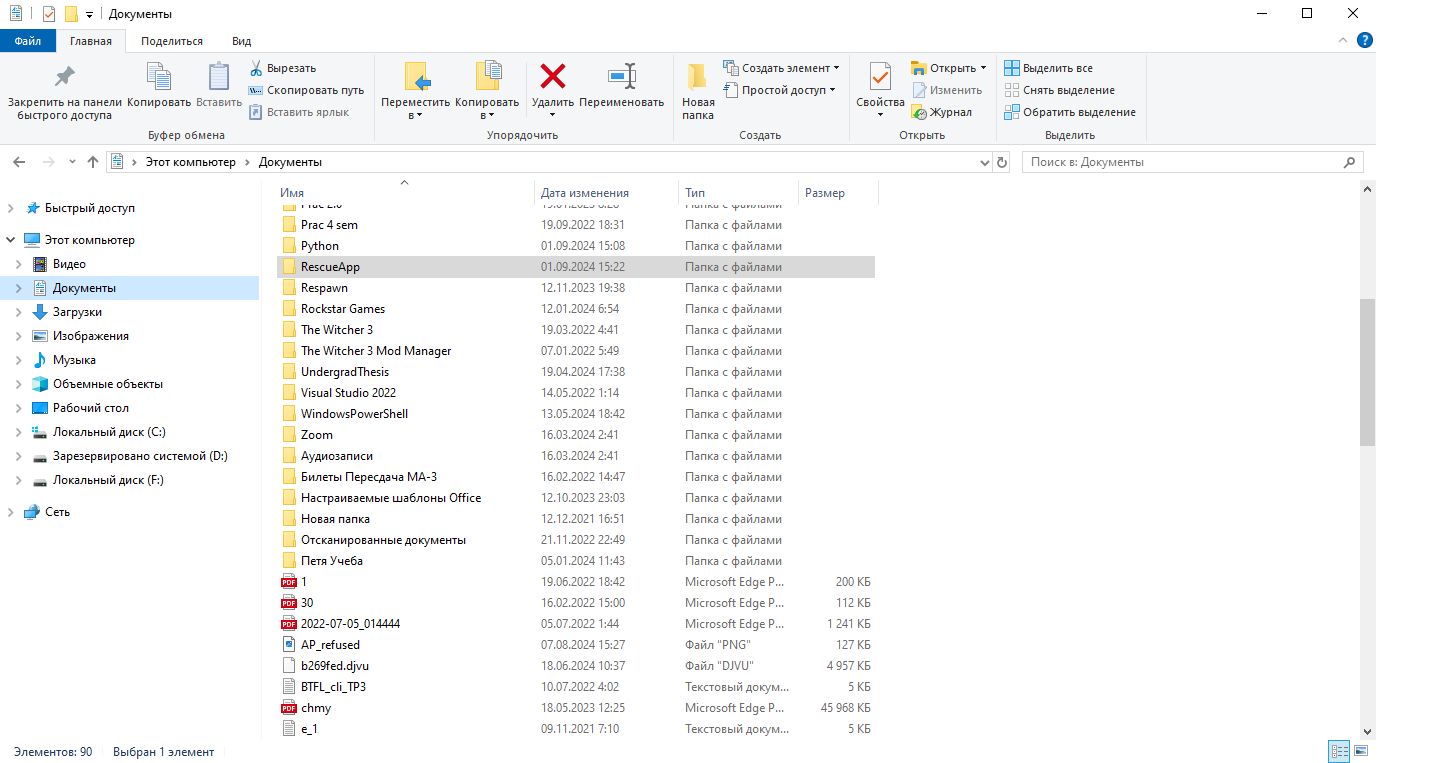
\includegraphics[width=\textwidth]{data_latex/tutor_pic1.png}  \\  }
\end{minipage}
\caption{Новая папка}
\end{figure}

После создания папки распаковываем архив и перемещаем содержимое в неё.

\subsection{Создание виртуальной среды}
\textbf{ВАЖНО! Шаги 1.3 - 1.5 нужны для того случая если не сработает вариант с батником 1.6, это возможно так как я никогда раньше не имел с ними дела и мб где-то накосячил. Так что сначала посмотрите его. }


Для изоляции зависимостей проекта от глобальных библиотек Python, рекомендуется создать виртуальную среду. Для этого откройте командную строку (CMD) и выполните следующие команды:

1. Перейдите в папку проекта:
   \begin{verbatim}
   cd Документы\RescueApp
   \end{verbatim}

2. Создайте виртуальную среду:
   \begin{verbatim}
   python -m venv venv
   \end{verbatim}

3. Активируйте виртуальную среду:
   \begin{verbatim}
   venv\Scripts\activate
   \end{verbatim}

После выполнения этих команд, вы увидите, что в командной строке появится префикс \texttt{(venv)}, что означает, что виртуальная среда активирована.

\subsection{Установка сторонних библиотек}
Теперь, когда виртуальная среда активирована, можно установить все необходимые сторонние библиотеки. Для этого выполните следующую команду:

\begin{verbatim}
pip install -r requirements.txt
\end{verbatim}

Файл \texttt{requirements.txt} должен находиться в папке проекта и содержать список всех необходимых библиотек.

\subsection{Запуск программы}
После установки всех библиотек, вы можете запустить программу, выполнив следующую команду:

\begin{verbatim}
python main.py
\end{verbatim}

Где \texttt{main.py} — это основной файл вашей программы.

\subsection{Использование батника для автоматизации}
Для удобства, можно использовать батник, который автоматически выполнит все необходимые шаги для установки и запуска программы. Для этого я создал файл `run\_program.bat`, и поместил его в папку проекта. Итого, для удобного запуска программы достаточно будет просто создать ярлык на рабочем столе, который открывает данный файл. Вот содержимое батника:

\begin{verbatim}
@echo off
REM Переходим в директорию проекта
cd /d %~dp0

REM Выводим текущий путь для отладки
echo Current path: %cd%

REM Проверяем наличие файла requirements.txt
if not exist requirements.txt (
    echo File requirements.txt not found!
    pause
    exit /b 1
)

REM Создаем виртуальную среду, если она еще не создана
if not exist venv (
    python -m venv venv
)

REM Активируем виртуальную среду
call venv\Scripts\activate

REM Устанавливаем необходимые библиотеки, если они еще не установлены
pip install -r requirements.txt

REM Запускаем программу
python main.py

REM Деактивируем виртуальную среду после завершения работы программы
deactivate

pause
\end{verbatim}

Достаточно просто запустить этот батник, чтобы установить все необходимые библиотеки и запустить вашу программу. 


\textbf{ПЕРВЫЙ ЗАПУСК МОЖЕТ ЗАНЯТЬ МНОГО ВРЕМЕНИ (до 5ти минут)}

\textbf{ЕСЛИ ПРИ ЗАПУСКЕ ДАЖЕ ПО ПРОШЕСТВИИ 5ТИ МИНУТ НИЧЕГО НЕ ПРОИСХОДИТ, МОЖНО ПОПРОБОВАТЬ ЗАПУСТИТЬ ФАЙЛ ОТ ИМЕНИ АДМИНИСТРАТОРА}

\textbf{ТАК ЖЕ АНТИВИРУСЫ МОГУТ НАЧАТЬ РУГАТЬСЯ НА БАТНИК, В ЭТОМ СЛУЧАЕ НАДО УЖЕ ПОСТУПАТЬ В ЗАВИСИМОСТИ ОТ КОНКРЕТНОГО АНТИВИРУСА (Касперский, например, долго его рассматривает, после чего помечает как безопасный и разрешает им пользоваться)}
\section{Инструкция к программе}
Сам интерфейс программы представляет из себя следующую менюшку, написанную на pyqt6 (рис. 2). Как видно, она состоит из 4х основных секций. Давайте по порядку рассмотрим каждую из них.
\begin{figure}[hbt!]
\begin{minipage}[h]{\linewidth}
\center{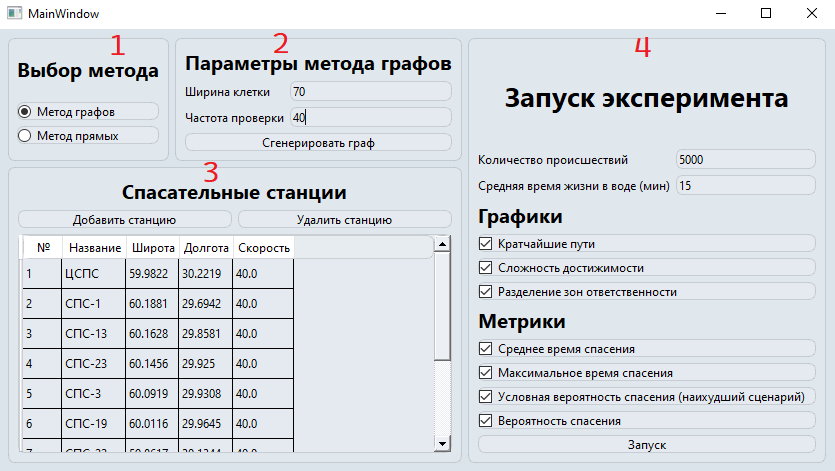
\includegraphics[width=\textwidth]{data_latex/tutor_pic4.png}  \\  }
\end{minipage}
\caption{Интерфейс программы}
\end{figure}

\subsection{Выбор метода} При реализации программы было рассмотрено два метода нахождения кратчайшего пути от спасательных станций до места ЧП --- метод прямых и метод графов. 
    \begin{itemize}
        \item \textbf{Метод прямых} --- быстрый, неточный метод, сильно специализированный под конкретный случай Финского залива. Этот метод был написан мной для того, чтобы свести к минимуму время, затрачиваемое на вычисление одного случая, он создан исключительно для получения приблизительных результатов и может показывать странные результаты для некоторых расстановок СПС (например, для маленького количества спасательных станций наблюдались ошибки, когда траектории спасательных бригад прокладывались задевая сушу). Если честно, не рекомендуется для получения визуальных картинок.
        \item \textbf{Метод графов} --- намного более точный, но в то же время ресурсоёмкий метод. Построен на основе алгоритма Дейкстры и дискретизации данного пространства. Этот метод более универсален и намного легче переносится на другие акватории, но в то же время требует больше времени для выполнения.
    \end{itemize}
\subsection{Параметры метода графов} Данный раздел доступен, очевидно, только при выбранном методе графов и позволяет более тонко настроить некоторые его параметры, такие как ширина клетки дискретизации и частота проверок пересечения суши. 
    \begin{itemize}
        \item \textbf{Ширина клетки} --- при прогоне алгоритма графов, всё пространство дискретизируется клетками определённой ширины (в пикселях, относительно карты "data/canvas\_new\_fish\_gray.png" с шириной 4113 и высотой 3145 пикселей). По умолчанию стоит значение 70, но для конечных расчётов это значение может быть грубовато, так что рабочий диапазон значений --- \textbf{$[20, 100]$}, где чем меньше значение, тем точнее результат, но программа работает дольше. 
        \item \textbf{Частота проверок пересечения суши} --- довольно неестественный параметр. Дело в том, что при формировании графа по всей длине каждой связи проводятся проверки типа "а проходит ли эта связь через кусок суши?". Так что данный параметр стоит трогать (увеличивать), только если на больших значениях ширины клетки (70+) заметны грубые ошибки по типу траекторий, нагло перепрыгивающих через кусок суши. В таком случае можно поднять этот параметр до 60 или даже выше. В противном случае параметр лучше не трогать.
    \end{itemize}
    Важная ремарка заключается в том, что расчёт графа с конкретными параметрами (особенно для маленькой ширины клеток) может занимать даже больше времени, чем сам эксперимент. Поэтому все посчитанные графы автоматически сохраняются в отдельную папку и при выставлении новой совокупности параметров, если граф с такими параметрами уже был посчитан, то программа не тратит время на его генерацию, а сразу подгружает его из памяти. Т.е. чтобы программа работала быстрее, нужно использовать уже ранее использованные совокупности параметров, например, \textbf{$\{70, 40\}$}, \textbf{$\{40, 40\}$} или \textbf{$\{20, 40\}$}.
    Кнопка "сгенерировать граф" запускает расчет графа с указанными параметрами и загружает его в библиотеку уже подготовленных графов без запуска самого эксперимента.

\subsection{Спасательные станции} В данном разделе всё просто --- тут представлен интерфейс для работы с самим расположением спасательных станций. У каждой станции есть несколько параметров: Название, координаты и скорость спасательного средства, доступного станции. По умолчанию в программу вписан список активных на данный момент спасательных станций, предоставленный мне спасательно-поисковой службой. Для добавления и удаления станций предусмотрены две кнопки. 
    \begin{itemize}
        \item \textbf{Добавление станции: } при нажатии данной кнопки открывается следующее диалоговое окно (рис. 3).
        \begin{figure}[hbt!]
            \begin{minipage}[h]{\linewidth}
                \center{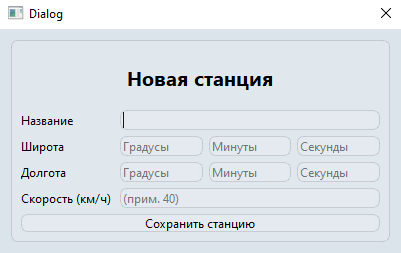
\includegraphics[width=0.55\textwidth]{data_latex/tutor_pic5.png}  \\  }
            \end{minipage}
            \caption{Добавление станции}
        \end{figure}
        Широту и долготу можно ввести двумя способами --- вписать дробные значения градусов (через точку, например 60.12) в первые колонки (градусы) оставив остальные поля пустыми, либо воспользоваться стандартным форматом градусы/минуты/секунды. В обоих случаях программа проверит правильность формата введенных данных, и если всё в порядке, добавит новую станцию в таблицу в секции 3.
        \item \textbf{Удаление станции: } при нажатии данной кнопки открывается следующее диалоговое окно (рис. 4).
        \begin{figure}[hbt!]
            \begin{minipage}[h]{\linewidth}
                \center{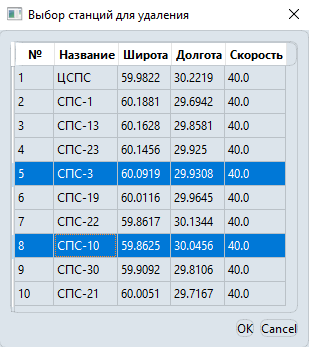
\includegraphics[width=0.55\textwidth]{data_latex/tutor_pic6.png}  \\  }
            \end{minipage}
            \caption{Удаление станции}
        \end{figure}
        В данной таблице можно нажатием мыши выбрать те станции, которые следует удалить, после чего нажать кнопку "ОК". Эти станции будут удалены из списка.
    \end{itemize}

\subsection{Запуск эксперимента} Это главная секция интерфейса, из которой, собственно, и запускается выполнение эксперимента. В ней мы рассмотрим следующие параметры.
    \begin{itemize}
        \item \textbf{Количество происшествий: } --- число случаев (точек), раскиданных по акватории. В математической статистике принято считать, что для метода Монте-Карло, используемого нами для расчета вероятности спасения, достоверный размер выборки должен составлять не менее $10000$ точек, тем не менее так как у нас не самая точная модель, количество точек можно снизить до $2000$ без значительной потери в точности, при этом ощутимо снизив время работы программы. 
        \item \textbf{Среднее время жизни в воде: } --- время, при котором абсолютное большинство людей, помещенных в данные экстремальные условия, погибнет. 
    \end{itemize}
    \subsubsection{Графики} 
    Тут можно выбрать, графики какого вида мы хотим увидеть на выходе работы программы. Пока добавлено всего три варианта: 
    \begin{itemize}
        \item Кратчайшие пути --- главный график (рис. 5), на котором отмечены спасательные станции и места сгенерированных ЧП, а так же изображены оптимальные траектории .
        \begin{figure}[hbt!]
            \begin{minipage}[h]{\linewidth}
                \center{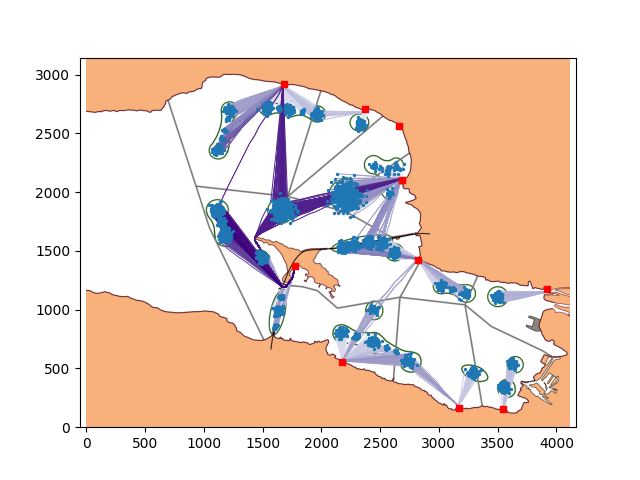
\includegraphics[width=0.8\textwidth]{data_latex/plot_example.png}  \\  }
            \end{minipage}
            \caption{Пример графика кратчайших путей}
        \end{figure}
        \item Сложность достижимости --- вспомогательный график (рис. 6). На нём с помощью тепловой карты отмечены труднодосягаемые участки акватории (чем темнее участок, тем дольше до него добираться из всех спасательных станций в совокупности). 
        \begin{figure}[hbt!]
            \begin{minipage}[h]{\linewidth}
                \center{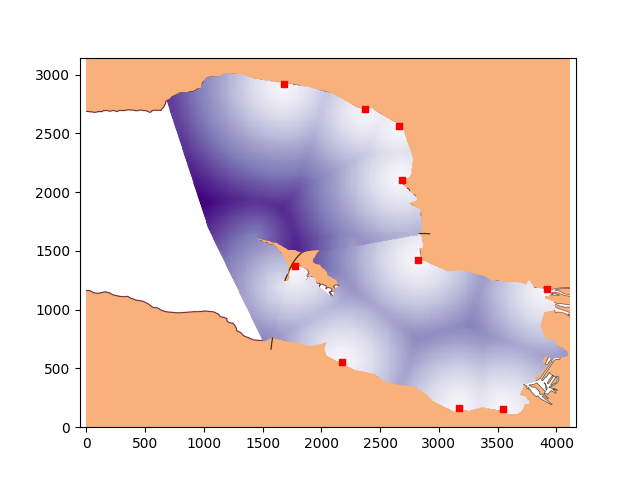
\includegraphics[width=0.8\textwidth]{data_latex/plot_reachability_example.png}  \\  }
            \end{minipage}
            \caption{Пример графика сложности достижимости}
        \end{figure}
        \item Распределение зон ответственности --- ещё один вспомогательный график (рис. 7). На нём вся акватория раскрашена в разные цвета радуги, каждый из которых соответствует зоне покрытия конкретной спасательной станции, размещённой на нём. То есть, например, внутри зоны зеленого цвета быстрее всего среагирует именно станция, расположенная в этой зоне. 
        \begin{figure}[hbt!]
            \begin{minipage}[h]{\linewidth}
                \center{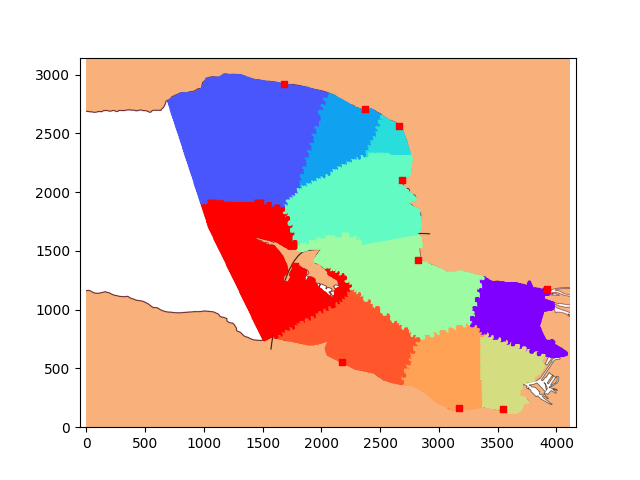
\includegraphics[width=0.8\textwidth]{data_latex/plot_reachability_difSt_example.png}  \\  }
            \end{minipage}
            \caption{Пример графика распределения зон ответственности}
        \end{figure}
    \end{itemize}
    \subsubsection{Метрики} 
    Тут уже всё тривиально, нужно выбрать те числовые значения, которые хочется вывести на экран в результате работы программы. Выводимое время реагирования показывается в минутах и \textbf{НЕ ВКЛЮЧАЕТ} в себя то время, которое требуется на подготовку экипажу к выходу.

    \subsubsection{Запуск программы}
    После нажатия на кнопку "Запуск" начинается выполнение вычислений и вывод полученных графиков. Это может занять некоторое время. К сожалению, я всё ещё работаю над тем, чтобы на время проведения вычислений кнопка "Запуск" меняла свой внешний вид и отключалась, поэтому пока следует обращать внимание на то, что не стоит несколько раз подряд нажимать на эту кнопку, так как это может привести к замедлению процесса (запустится сразу несколько экспериментов). 

    Окна с полученными результатами экспериментов не закрываются после запуска новых его итераций, так что для большей наглядности можно запустить эксперимент, получить результат, поменять данные (например, изменить параметры графа или добавить ещё станции) и запустить эксперимент снова. В результате будет открыто два окна с результатами, которые можно будет поставить бок о бок и сравнивать друг с другом, что довольно удобно. 

\end{document}
